\begin{figure}[htbp]
  \centering
  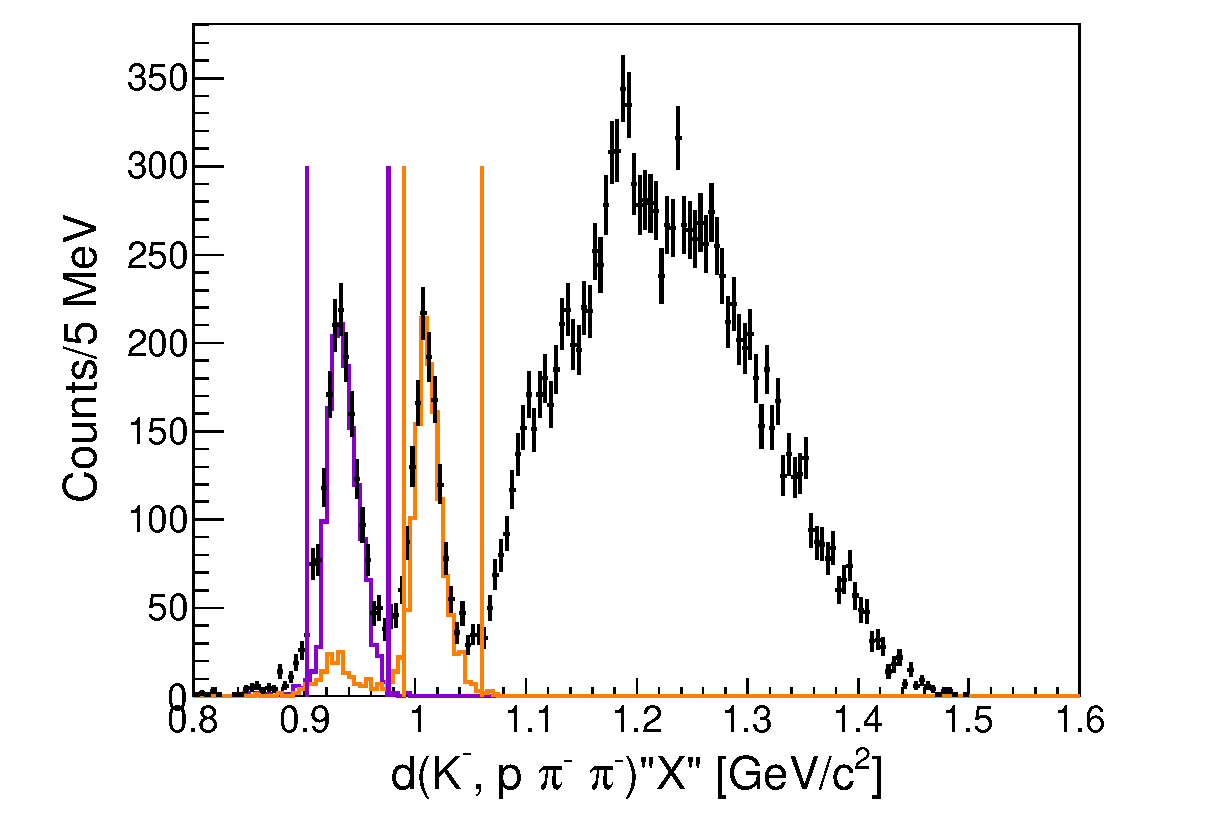
\includegraphics[width=8cm]{../pic/Run68/KP_ana/KPpimpim_MM.eps}
  \caption{
    This figure shows the missing mass of $d(K^-, p \pi^- \pi^-)$.
    Orange and purple lines indicate selection region as missing $p$ and $p \pi^-$, respectively.
    $d(K^-, p \pi^-)"\Sigma^0"$ and $d(K^-, p \pi^-)"\Lambda"$ tagged events are drawn orange and purple plot in same figure.
  }
  \label{fig:KPpimpim}
\end{figure}
